%%%%%%%%%%%%%%%%%%%%%%%%%%%%%%%%%%%%%%%%%%%%%%%%%%%%%%%%%%
%   Vorlage von:
%
%   Prof. Dr. Bernhard Drabant
%   Prof. Dr. Dennis Pfisterer
%   Prof. Dr. Julian Reichwald
%
%%%%%%%%%%%%%%%%%%%%%%%%%%%%%%%%%%%%%%%%%%%%%%%%%%%%%%%%%%

%%%%%%%%%%%%%%%%%%%%%%%%%%%%%%%%%%%%%%%%%%%%%%%%%%%%%%%%%%
%	ANLEITUNG: 
%
%   1. Ersetzen Sie firmenlogo.jpg im Verzeichnis img
%   2. Passen Sie alle Stellen im Dokument an, die mit 
%      @stud markiert sind
%
%%%%%%%%%%%%%%%%%%%%%%%%%%%%%%%%%%%%%%%%%%%%%%%%%%%%%%%%%%

%%%%%%%%%%%%%%%%%%%%%%%%%%%%%%%%%%%%%%%%%%%%%%%%%%%%%%%%%%
%	ACHTUNG: 
%
%   Für das Erstellen des Literaturverzeichnisses wird das 
%   modernere Paket biblatex in Kombination mit biber 
%   verwendet -- nicht mehr das ältere BibTex!
%   Bitte stellen Sie ggf. Ihre TeX-Umgebung entsprechend 
%   ein (z.B. TeXStudio: Einstellungen --> Erzeugen --> 
%   Standard Bibliographieprogramm: biber)
%
%%%%%%%%%%%%%%%%%%%%%%%%%%%%%%%%%%%%%%%%%%%%%%%%%%%%%%%%%%

\documentclass[fontsize=12pt,BCOR=5mm,DIV=12,
               parskip=half,
               listof=entryprefix,paper=a4,toc=bibliography,toc=listof,pointlessnumbers
               %,headinclude=on,footinclude=off,
               %,plainheadtopline=false,plainheadsepline=false,plainfootsepline=false,plainfootbotline=false
               ]{scrreprt}
               
\makeindex

% (!!) Elementare Pakete, Konfigurationen und Definitionen werden geladen
% !TEX root =  master.tex
%      HYPERREF

%%%%%%%%%%%%%%%%%%%%%%%%%%%%%%%%%%%%%%%%%%%%%%%%%%%%%%%%%%
%	ANLEITUNG: 
%
% Passen Sie alle Stellen im Dokument an, die mit 
% @stud markiert sind
%
%%%%%%%%%%%%%%%%%%%%%%%%%%%%%%%%%%%%%%%%%%%%%%%%%%%%%%%%%%
\usepackage{listings}
\usepackage{makeidx}         % allows index generation
\usepackage{listings}	%Format Listings properly
\usepackage{lipsum}    %Blindtext
\usepackage{graphicx} % use various graphics formats
\usepackage[german]{varioref} 	% nicer references \vref
\usepackage{caption}	%better Captions
\usepackage{booktabs} %nicer Tabs
\usepackage{array}
\usepackage{chngcntr}
\usepackage[hidelinks=true]{hyperref} % keine roten Markierungen bei Links
\usepackage{fnpct} % Correct superscripts 
\usepackage[T1]{fontenc}
\usepackage[utf8]{inputenc}
\usepackage{calc} % Used for extra space below footsepline
\usepackage{acronym}
\usepackage{algorithm}
\usepackage{algpseudocode}
\usepackage{setspace}

%
% @stud
%
%	FONT SELECTION: Entweder 1) Latin Modern oder 2) Times / Helvetica
\usepackage{lmodern}             % 1) Latin modern font
%\usepackage{mathptmx}           % 2) Helvetica / Times New Roman fonts (2 lines)
%\usepackage[scaled=.92]{helvet} % 2) Helvetica / Times New Roman fonts (2 lines)

%
% @stud
%
%	LANGUAGE SETTINGS
\usepackage[ngerman]{babel} 	        % german language
\usepackage[german=quotes]{csquotes} 	% correct quoting using \enquote{}
%\usepackage[english]{babel}          % english language
%\usepackage{csquotes} 	              % correct quoting using \enquote{}

%
% @stud
%
% Uncomment the following lines to support hard URL breaks in bibliography 
%\apptocmd{\UrlBreaks}{\do\f\do\m}{}{}
%\setcounter{biburllcpenalty}{9000}% Kleinbuchstaben
%\setcounter{biburlucpenalty}{9000}% Großbuchstaben

%
% @stud
%
%	FOOTNOTES: Count footnotes over chapters
%1 \counterwithout{footnote}{chapter}

%	ACRONYMS
\makeatletter
\@ifpackagelater{acronym}{2015/03/20}
{\renewcommand*{\aclabelfont}[1]{\textbf{{\acsfont{#1}}}}}{}
\makeatother

%	LISTINGS
\renewcommand{\lstlistingname}{Quelltext} 
\renewcommand{\lstlistlistingname}{Quelltextverzeichnis}
\lstset{numbers=left,
	numberstyle=\tiny,
	captionpos=b,
	basicstyle=\ttfamily\small}

%	ALGORITHMS
\renewcommand{\listalgorithmname}{Algorithmenverzeichnis }
\floatname{algorithm}{Algorithmus}

%		PAGE HEADER / FOOTER
%	    Warning: There are some redefinitions throughout the master.tex-file!  DON'T CHANGE THESE REDEFINITIONS!
\RequirePackage[automark]{scrlayer-scrpage}
%alternatively with separation lines: \RequirePackage[automark,headsepline,footsepline]{scrlayer-scrpage}

%\renewcommand*{\pnumfont}{\upshape\sffamily}
%\renewcommand*{\headfont}{\upshape\sffamily}
%\renewcommand*{\footfont}{\upshape\sffamily}

\renewcommand{\chaptermarkformat}{}
\RedeclareSectionCommand[beforeskip=0pt]{chapter}
\clearscrheadfoot

%\ifoot[\rule{0pt}{\ht\strutbox+\dp\strutbox}DHBW Mannheim]{\rule{0pt}{\ht\strutbox+\dp\strutbox}DHBW Mannheim}
\ofoot[\rule{0pt}{\ht\strutbox+\dp\strutbox}\pagemark]{\rule{0pt}{\ht\strutbox+\dp\strutbox}\pagemark}
\ohead{\headmark}

\newcommand{\TitelDerArbeit}[1]{\def\DerTitelDerArbeit{#1}\hypersetup{pdftitle={#1}}}
#\newcommand{\AutorDerArbeit}[1]{\def\DerAutorDerArbeit{#1}\hypersetup{pdfauthor={#1}}}
\newcommand{\DerAutorDerArbeitEins}[1]{\def\DerAutorDerArbeitEins{#1}\hypersetup{pdfauthor={#1}}}
\newcommand{\DerAutorDerArbeitZwei}[1]{\def\DerAutorDerArbeitZwei{#1}\hypersetup{pdfauthor={#1}}}
\newcommand{\DerAutorDerArbeitDrei}[1]{\def\DerAutorDerArbeitDrei{#1}\hypersetup{pdfauthor={#1}}}
\newcommand{\DerAutorDerArbeitVier}[1]{\def\DerAutorDerArbeitVier{#1}\hypersetup{pdfauthor={#1}}}
\newcommand{\Firma}[1]{\def\DerNameDerFirma{#1}}
\newcommand{\Kurs}[1]{\def\DieKursbezeichnung{#1}}
\newcommand{\Abteilung}[1]{\def\DerNameDerAbteilung{#1}}
\newcommand{\Studiengangsleiter}[1]{\def\DerStudiengangsleiter{#1}}
\newcommand{\WissBetreuer}[1]{\def\DerWissBetreuer{#1}}

\newcommand{\Bearbeitungszeitraum}[1]{\def\DerBearbeitungszeitraum{#1}}
\newcommand{\Abgabedatum}[1]{\def\DasAbgabedatum{#1}}
\newcommand{\Matrikelnummer}[1]{\def\DieMatrikelnummer{#1}}
\newcommand{\Studienrichtung}[1]{\def\DieStudienrichtung{#1}}
\newcommand{\ArtDerArbeit}[1]{\def\DieArtDerArbeit{#1}}
\newcommand{\Literaturverzeichnis}{Literaturverzeichnis}

\newcommand{\settingBibFootnoteCite}{
	\setlength{\bibparsep}{\parskip}		  % Add some space between biblatex entries in the bibliography
	\addbibresource{bibliography.bib}	    % Add file bibliography.bib as biblatex resource
	\DefineBibliographyStrings{ngerman}{andothers = {{et\,al\adddot}},}
	\AdaptNoteOpt\footcite\multfootcite   % Will add  separators if footcite is called multiple consecutive times 
	\AdaptNoteOpt\autocite\multautocite   % Will add  separators if autocite is called multiple consecutive times
}

\newcommand{\setTitlepage}{
	% !TEX root =  master.tex
\begin{titlepage}
\begin{minipage}{\textwidth}
		\vspace{-2cm}
		\noindent \hfill 
\includegraphics{\imagedir/logo.jpg}
\end{minipage}
\vspace{1em}
%\sffamily
\begin{center}
	{\textsf{\large Duale Hochschule Baden-W\"urttemberg Mannheim}}\\[4em]
	{\textsf{\textbf{\large{\DieArtDerArbeit}arbeit}}}\\[6mm]
	{\textsf{\textbf{\Large{}\DerTitelDerArbeit}}} \\[1.5cm]
	{\textsf{\textbf{\large{}Studiengang Wirtschaftsinformatik}}\\[6mm]
	\textsf{\textbf{Studienrichtung \DieStudienrichtung}}}\vspace{10em}
	
	\begin{minipage}{\textwidth}
		\begin{tabbing}
		Wissenschaftlicher Betreuer: \hspace{0.85cm}\=\kill
		Verfasser und Matrikelnummer: \> \DerAutorDerArbeitEins \\[1.5mm]
		\> \DerAutorDerArbeitZwei \\[1.5mm]
		\> \DerAutorDerArbeitDrei \\[1.5mm]
		\> \DerAutorDerArbeitVier \\[1.5mm]
		Kurs: \> \DieKursbezeichnung \\[1.5mm]
		Studiengangsleiter: \> \DerStudiengangsleiter \\[1.5mm]
		Wissenschaftlicher Betreuer: \> \DerWissBetreuer \\[1.5mm]
		Bearbeitungszeitraum: \> \DerBearbeitungszeitraum\\[1.5mm]
%		alternativ:\\[1.5mm]
%		Eingereicht: \> \DasAbgabedatum	
		\end{tabbing}
	\end{minipage}
\end{center}
\end{titlepage}
	\pagenumbering{roman} % Römische Seitennummerierung
	\normalfont	
}

%
% @stud
%
\newcommand{\settingLists}{
	%	Inhaltsverzeichnis
	\tableofcontents
	%	Abbildungsverzeichnis
	\listoffigures
	%	Tabellenverzeichnis
	\listoftables
	%	Listingsverzeichnis / Quelltextverzeichnis
	\lstlistoflistings
	% Algorithmenverzeichnis
	\listofalgorithms
}

\newcommand{\initializeText}{
	\clearpage
	\ihead{\chaptername~\thechapter} % Neue Header-Definition
	\pagenumbering{arabic}           % Arabische Seitenzahlen
}

\newcommand{\initializeBibliography}{
	\ihead{}
	\printbibliography[title=\Literaturverzeichnis] 
	\cleardoublepage
}

\newcommand{\initializeAppendix}{
	\appendix
	\ihead{\appendixname~\thechapter}
}



%%%%%%%%%%%%%%%%%%%%%%%%%%%%
%
% @stud
%
%	SCHRIFTART (Schrift mit oder ohne Serifen im gesamten Text) 
%
% mit Serifen
%\addtokomafont{disposition}{\rmfamily}
%\renewcommand*{\familydefault}{\rmdefault}
%
% ohne Serifen (default)
%\addtokomafont{disposition}{\sffamily}
%
%%%%%%%%%%%%%%%%%%%%%%%%%%%%

%%%%%%%%%%%%%%%%%%%%%%%%%%%%
%
% @stud
%
% PERSÖNLICHE ANGABEN (BITTE VOLLSTÄNDIG EINGEBEN zwischen den Klammern: {...})
%
\ArtDerArbeit{Seminar} % "Bachelor" oder "Projekt" wählen
\TitelDerArbeit{Intelligente Spur- und Objekterkennung als Teil des autonomen Fahrens}
\DerAutorDerArbeitEins{Andreas Bernrieder - 7876007}
\DerAutorDerArbeitZwei{Thorsten Hilbradt - 5034067}
\DerAutorDerArbeitDrei{Jan Brebeck - 8016697}
\DerAutorDerArbeitVier{Simon Scapan - 6699329}
\Kurs{WWI18DSB}
\Studienrichtung{Data Science}
\Studiengangsleiter{Prof. Dr. Bernhard Drabant}
\WissBetreuer{Prof. Dr. Bernhard Drabant}
\Bearbeitungszeitraum{01.12.2020 -- 25.01.2021}
\Abgabedatum{25.01.2021}
%
%%%%%%%%%%%%%%%%%%%%%%%%%%%%

%%%%%%%%%%%%%%%%%%%%%%%%%%%%
%
% @stud
%
%	BIBLIOGRAPHY (@stud: Bibliographie-Stil wählen - Position und Indizierung)
%
% Auswahl zwischen: IEEE Style, ALPHABETIC Style, HARVARD Style, AUTHOR-YEAR Style 
%
% (oder eigenen zulässigen Stil wählen) 
%

% Position des Zitats
%
\newcommand{\position}{inline} 
%\newcommand{\position}{footnote}

% Indizierung des Zitats
%
% 1) NUMERIC Style - e. g. [12]
\newcommand{\indextype}{numeric} 
%
% 2) ALPHABETIC Style - e. g. [AB12]
%\newcommand{\indextype}{alphabetic} 
%
% 3) IEEE Style - numeric kind of style 
%\newcommand{\indextype}{ieee} 
%
% 4) HARVARD Style 
%\newcommand{\indextype}{apa} 
%
% 5) CHICAGO Style 
%\newcommand{\indextype}{authoryear}
%
%%%%%%%%%%%%%%%%%%%%%%%%%%%%

\renewcommand*{\familydefault}{\sfdefault}

\usepackage[backend=biber, autocite=\position, style=\indextype]{biblatex} 	

\settingBibFootnoteCite

\newcommand{\abs}{\par\vskip 0.2cm\goodbreak\noindent}
\newcommand{\nl}{\par\noindent}
\newcommand{\mcl}[1]{\mathcal{#1}}
\newcommand{\nowrite}[1]{}
\newcommand{\NN}{{\mathbb N}}

\newcommand{\imagedir}{img}

\makeindex

\begin{document}

\setTitlepage

%%%%%%%%%%%%%%%%%%%%%%%%%%%%%%%%%%%%%%%%%%%%%%%%%%%%%%%%%%%%%%%%%%%%%%%%%%%%%%%%%%%%%%%%%%
% KAPITEL UND ANHÄNGE
%
% @stud:
%   - nicht benötigte: auskommentieren/löschen
%   - neue: bei Bedarf hinzufügen mittels input-Kommando an entsprechender Stelle einfügen
%%%%%%%%%%%%%%%%%%%%%%%%%%%%%%%%%%%%%%%%%%%%%%%%%%%%%%%%%%%%%%%%%%%%%%%%%%%%%%%%%%%%%%%%%%

%%%%%%%%%%%%%%%%%%%%%%%%%%%%%%%%%%%
% EHRENWÖRTLICHE ERKLÄRUNG
%
% @stud: ewerkl.tex bearbeiten
%
% !TEX root =  master.tex
\clearpage
\chapter*{Ehrenwörtliche Erklärung}

% Wird die folgende Zeile auskommentiert, erscheint die ehrenwörtliche
% Erklärung im Inhaltsverzeichnis.

% \addcontentsline{toc}{chapter}{Ehrenwörtliche Erklärung}
Wir versicheren hiermit, dass wir die vorliegende Arbeit
 mit dem Thema: \textit{\DerTitelDerArbeit} selbstständig verfasst und keine anderen als die angegebenen Quellen und
Hilfsmittel benutzt haben. Wir versicheren zudem,
dass die eingereichte elektronische Fassung mit der gedruckten Fassung übereinstimmt.

\vspace{3cm}
Ort, Datum \hfill \DerAutorDerArbeit
 
%%%%%%%%%%%%%%%%%%%%%%%%%%%%%%%%%%%

%%%%%%%%%%%%%%%%%%%%%%%%%%%%%%%%%%%
% SPERRVERMERK
%
% @stud: nondisclosurenotice.tex bearbeiten
%
%%%%%%%%%%%%%%%%%%%%%%%%%%%%%%%%%%%

%%%%%%%%%%%%%%%%%%%%%%%%%%%%%%%%%%%
%	KURZFASSUNG
%
% @stud: acknowledge.tex bearbeiten
%
%% !TEX root =  master.tex
\chapter*{Danksagung}

Hier können Sie eine Danksagung schreiben. 


 
%%%%%%%%%%%%%%%%%%%%%%%%%%%%%%%%%%%

%%%%%%%%%%%%%%%%%%%%%%%%%%%%%%%%%%%
%	KURZFASSUNG
%
% @stud: abstract.tex bearbeiten
%
% !TEX root =  master.tex
\chapter*{Abstract}

Hier können Sie die Kurzfassung (engl.~Abstract) der Arbeit schreiben. Beachten Sie dabei die Hinweise zum Verfassen der Kurzfassung.


 
%%%%%%%%%%%%%%%%%%%%%%%%%%%%%%%%%%%

%%%%%%%%%%%%%%%%%%%%%%%%%%%%%%%%%%%
% VERZEICHNISSE
%
% @stud: ggf. nicht benötigte Verzeichnisse auskommentieren/löschen in Def. von \settingLists in config.tex
%
\settingLists
%%%%%%%%%%%%%%%%%%%%%%%%%%%%%%%%%%%

%%%%%%%%%%%%%%%%%%%%%%%%%%%%%%%%%%%
% ABKÜRZUNGSVERZEICHNIS
%
% @stud: acronyms.tex bearbeiten
%
% !TEX root =  master.tex
\clearpage
\chapter*{Abkürzungsverzeichnis}	
\addcontentsline{toc}{chapter}{Abkürzungsverzeichnis}

\begin{acronym}[XXXXXXX]
	\acro{DHBW}{Duale Hochschule Baden-Württemberg}
	\acro{OD}{Object Detection}
	\acro{OpenCV}{Open Source Computer Vision Library}
	\acro{LiDAR}{Light Detection And Ranging}
	\acro{YOLO}{You Only Look Once}
	\acro{OR}{Object Recognition}
	\acro{OC}{Object Classification}
	\acro{CNN}{Convolutional Neural Network}
	\acro{R-CNN}{Region-based Convolutional Network}
	\acro{SVM}{Support Vector Machine}
	\acro{FPS}{Frames per Second}
	\acro{SSD}{Single Shot MultiBox Detector}
	\acro{Pi}{Raspberry Pi}
	\acro{GPIO}{General Purpose Input/Output}
	\acro{SELMA}{\textbf{Sel}bstfahrendes \textbf{M}odell\textbf{a}uto}
	\acro{PWM}{Pulsweitenmodulation}
	\acro{LD}{Lane Detection}
	\acro{GPS}{Global Positioning System}
	\acro{RGB}{Grundfarben: Rot, Grün und Blau}
	\acro{DCNN}{Deep Convolutional Neural Network}
	\acro{DRNN}{Deep Recurrent Neural Network}
	\acro{LSTM}{Long Short Term Memory}
	
\end{acronym} 
%%%%%%%%%%%%%%%%%%%%%%%%%%%%%%%%%%%

\initializeText
\onehalfspacing

%%%%%%%%%%%%%%%%%%%%%%%%%%%%%%%%%%%
% KAPITEL
%
% @stud: einzelne Kapitel bearbeiten und eigene Kapitel hier einfügen
%
% Einleitung
% !TEX root =  master.tex
\chapter{Einleitung}

In dieser wissenschaftlichen Arbeit wird sich mit dem Projekt der \enquote{Intelligente Spur- und Objekterkennung als Teil des autonomen Fahrens} beschäftigt.
Dieses Projekt ist Teil des Integrationsseminar an der \ac{DHBW} Mannheim im Wintersemester 2020/21.

Das Ziel des Projektes ist es ein System zu Entwickeln welches es ermöglicht Spuren und Objekten auf Bildern zu erkennen.
In der Planungsphase wurde sich dafür entschieden eine reale Umsetzung des Projektes mithilfe eines 1:10 ferngesteuertes Modellauto durchzuführen.
Um dies Umzusetzen muss das System so kompakt gebaut werden, dass ein RaspberryPi 3b+ die Ausführung des System bewältigen kann. 

Die verwendeten Algorithmen und Methoden belaufen sich auf \ac{YOLO} für die Objekterkennung. Für die Spurerkennung werden verschiedene Methoden der \ac{OpenCV} Programmierbibliothek verwendet.

\ac{YOLO} ist ein Algorithmus welcher eine abgewandelte Version eines \ac{CNN} verwendet um in einer Kürzeren zeit Objekte zu erkennen. 
Die genau Implementierung und Verwendung des \ac{YOLO} Algorithmus wird im Laufe der Arbeit detailliert beschrieben. 
Zusätzlich zu Objekterkennung wird hier auch die Entfernung zu den erkannten Objekten errechnet.

Die Spurerkennug ist basiert auf der \ac{OpenCV} Bibliothek. \ac{OpenCV} stellt viele verschiedene Algorithmen und Methoden zur Verfügung um Computer Vision umzusetzen. 
Welche Methoden und Algorithmen verwendet wurden wird in einem Kapitel genau beschrieben.

Die Vorgehensweise wie das Modellauto präpariert und modifiziert wurde um die Steuerung durch die Algorithmen zu ermöglichen wird in einem Abschließendem Kapitel beschrieben und dargestellt.
Dazu wird ebenfalls eine Anleitung bereitgestellt welche das verwenden der Systemem beschreibt.



% mehrere Grundlagen- und Forschungs-Kapitel
\chapter{OpenCV} % Kommentar Simon: ich würd's in der Tat 'OpenCV' nennen, da 'Computer Vision' ein Oberbegriff ist.



\section{Einleitung}
Die Computer Vision ist ein zentrales Element für diese Projekt, da es für den Computer möglich gemacht werden muss seine Umgebung zu erkennen.
Die Computer Vison kann beschrieben werden als der Weg des Bild in den Computer und wie ein Computer sehen kann. \cite{Priese2015}

Im verlauf des Projekts wird \ac{OpenCV} für die Objekterkennung sowie die Spurerkennung verwendet.
\ac{OpenCV} besteht aus mehr als 2500 optimierten Algorithmen zu Computer Vision und Machine Learning. 
Diese Algorithmen können verwendet werden um Gesichter zu erkennen, bestimmte Objekte zu erkennen und sich bewegende Objekte zu folgen. 
Diese ist lediglich ein kleiner Ausschnitt dessen was mit den fortschrittlichen Algorithmen der \ac{OpenCV} möglich ist.   \cite{OpenCV.2020}  



Kapitel enthält: Einführung in Computer Vision im Allgemeinen und in opencv (cv2) im speziellen.
benutzt für lane detction und object detection


\section{Grayscaling}\label{sec:greyscaling} % max 1 seite
- Grayscaling benötigen wir, um Farben aus dem Bild zu nehmen
- durch dadurch sind Farben nicht mehr in 3 verschiedenen Farbtiefen also in RGB mit jeweils 255 ausprägungen, sondern nur balck in 255 ausprägungen
- jetzt können wir also nur noch durch kontraste verschiedene Elemente im Bild erkennen
- Das hilft uns, da wir nicht von vorn herein sagen können, welche Farbe die Fahrbahnbegrenzung haben wird, damit wir uns darauf fixieren können
- in Baustellenbereichen zum bleistift wird meist eine Gelbe MArkierung, also abweichend von einer weißen benutzt

- mal nachforschen ob kontraste im grayscale stärker sind als im Farbigen

- die weitere Berechnung wird aufgrund der fehlenden Farbtiefe und somit zusätzlicher Parameter verringert
- das bringt einen vorteil in der geschwindigkeit der berechnung und somit auch performance des gesamtsystems

- um das Bild zu transformieren wird die Methode cvtColor aus openCV genutzt, dabei wird das übergebene Bild mit dem Befehl cv2.COLOR\_RGB2GRAY vom RGB spektrum auf ein grau Spektrum herunter gebrochen


\section{Gaußsche Unschärfe} % max 1%

- cv2.GaussianBlur ... das ist die Funktion die ich im Code benutze
- das Bild wird quasi unscharf gemacht und die Farben glaube irgendwie bearbeitet aber lies das gern noch einmal nach

% https://docs.opencv.org/4.5.0/dd/d1a/group__imgproc__feature.html#ga04723e007ed888ddf11d9ba04e2232de

\section{Canny Transformation} % 1 - 2 seiten
 
- im code : cv2.Canny

das mit dem Canny ist in der Tat ziemlich wichtig ... das solltest du bisschen ausführlicher machen ... also dass irgendwie kontrastlinien erkannt werden und so dies das ... hab ich selbst nicht ganz verstanden, was da vor geht

\section{Hough Transformation} % 1-2 Seiten

% hough_lines(img, rho, theta, threshold, min_line_len, max_line_gap)

im code: cv2.HoughLinesP()

die hough transformation erkennt dann die vom canny gezeichneten linien und legt geraden drauf ... prinzip ist wieder klar aber wie das genau geht kann ich dir wieder nicht sagen ... da muss wieder literaturrecherche ran

\section{Fazit}

\chapter{Spur Erkennung}
%Simon


\section{Einführung} %0.5 Seiten
Die wichtigste Funktionalität beim autonomen Fahren ist die Spurerkennung und die damit einhergehende Steuerung des Fahrzeugs in dem Bereich der Fahrbahnlinien. Das Forschungsgebiet wird unter dem englischen Begriff \ac{LD} zusammengefasst. Es gibt mehrere möglichkeiten die Fahrbahnlinien zu erkennen. 
Dabei spielt die Beschaffenheit der Fahrbahn eine oft ungeahnt wichtige Rolle. Im Projekt wurde die Lane Detection zuerst in der Wohnung zweier Teammitglieder getestet. Dafür wurden Fahrspuren mit weisem Klebeband auf dem Boden markiert. Die Spurerkennung hat dabei gute Ergebnisse geliefert, da der Kontrast zwischen Boden und Markierung hoch war. Als dann aber zum ersten mal auf einem öffentlichen Parkplatz getestet wurde, war festzustellen, dass weise Körner im Asphalt bei so geringer Distanz zur Fahrbahn große Schwierigkeiten bergen. Deshalb wurde die Entschiedung für dieses Projekt getroffen zwischen zwei Terrains zu unterscheiden und die Spurerkennung darauf zu optimieren. Das ist zum einen die Strecke in der Wohnung aber auch die asphaltierte Fahrbahn auf dem Parkplatz.

Es gibt unterschiedliche Ansätze und Modelle, wie eine Fahrbahnlinienerkennung implementiert werden kann. Zum einen durch den Einsatz von Künsltichen Intelligenzen, welche anhand gelernter Datensätze neue Spuren erkennen und zum anderen gibt es den Ansatz Fahrspuren allein mit Hilfe Bildbearbeitender Wekrzeuge zu erkennen. Da schon tiefgreifendes Wissen im Bereich der Bildbearbeitung im Team vorhanden war wurde dieses Prinzip weiter verfolgt.

In den folgenden Unterkapiteln wird auf die verschiedenen Möglichkeiten der Spurerkennung eingegangen, dabei ins besondere auf die Python Bibliothek OpenCV. Aufbauend auf diesen Grundlagen wird dann die Datenstrecke implementiert und erläutert um am Ende diesen Kapitels den Wert für die Steuerung zu berechnen.


\section{State of the Art der Spur Erkennung} %0.5 Seiten
Für die Spurerkennung werden, wie bei der Objekterkennung im Regelfall mehrere Informationsquellen verarbeitet. Das sind vor allem Kamera- und Sensordaten aber auch Informationen über das \ac{GPS} wo sich das Fahrzeug zur Zeit befindet. Für dieses Projekt werden ausschließlich Kameradaten verwendet, was sich bei der Auswahl der Modelle widerspiegelt.

Wie in der Einführung in dieses Kapitel bereits angemerkt, kann für die Spurerkennung ein rein Bildbearbeitender Ansatz oder maschinelles Lernen genutzt werden. Beide Bereiche werden folgt erläutert.

\subsection{Umsetzung anhand maschinellem Lernen}
In diesem unterkapitel wird die Lane Detection mit einem Ansatz des maschinellen Lernen betrachtet. Im Detail wird auf einen Ansatz im Bereich des Supervised Learning gesetzt.
Der Hintergrund dessen ist, dass eine Szene nicht einzeln betrachtet werden kann. Wenn nur eine einzelne Momentaufnahme herangezogen wird um eine Entscheidung zu treffen wird diese schlechter ausfallen als wenn zusätzlich in die Vergangenheit geschaut wird. \cite{cnnld.2020}
Das heißt im Detail, dass zum Beispiel das aktuelle Bild analysiert wird und dazu die letzten drei, jedoch mit einer geringeren Gewichtung. Damit kann das Ziel erreicht werden, Fehler in der Erkennung zu vermeiden, da aus den vorherigen Inputdaten der Verlauf der Straße hervorgeht und der aktuelle Input dann die jüngste Veränderung aufweist. Die Notwendigkeit kann multipel begründet werden. Zum einen kann die Fahrbahnmarkierung verschmutzt oder durch Fahrzeuge und Gegenstände unterbrochen sein, in den meisten Fällen sind es jedoch Schatten, schlechte Lichtverhältnisse, Tunnel aber vor allem dreck auf der Straße.

Es gibt hauptsächlich zwei Arten von Deep Neural Networks. Zum einen Deep Convolutional Neural Network (DCNN), welches Inputdaten häufig mit mehreren Stufen der Convolution verarbeitet und gut geeignet für die Abstraktion von Merkmalen für Bilder und Videos ist. Zum anderen das Deep Recurrent Neural Network (DRNN), das Inputsignale rekursiv verarbeitet, indem es es in aufeinanderfolgende Blöcke aufteilt und vollständige Verbindungsschichten zwischen ihnen für die Statusausbreitung aufbaut. Die Vorteile zeigen sich bei der Vorhersage von Informationen für Zeitreihendaten.\cite{cnnld.2020}

-----------
Basierend auf der obigen Diskussion wird ein hybrides tiefes neuronales Netzwerk zur Spurerkennung unter Verwendung mehrerer kontinuierlicher Fahrszenenbilder vorgeschlagen. Das vorgeschlagene hybride tiefe neuronale Netzwerk kombiniert das DCNN und das DRNN. In einer globalen Perspektive ist das vorgeschlagene Netzwerk ein DCNN, der mehrere Rahmen als Eingabe verwendet und die Spur des aktuellen Rahmens auf semantische Segmentierungsweise vorhersagt. Eine vollständig gefaltete DCNN-Architektur wird vorgestellt, um das Segmentierungsziel zu erreichen. Es enthält ein Encoder-Netzwerk und ein Decoder-Netzwerk, die garantieren, dass die endgültige Ausgabekarte dieselbe Größe wie das Eingabebild hat. In einer lokalen Perspektive werden vom Encodernetzwerk von DCNN abstrahierte Merkmale von einem DRNN weiterverarbeitet. Ein LSTM-Netzwerk (Long Short Term Memory) wird verwendet, um die Zeitreihen codierter Merkmale zu verarbeiten. Der Ausgang von DRNN soll die Informationen der kontinuierlichen Eingangsrahmen zusammengeführt haben und wird in das Decodernetz des DCNN eingespeist, um die Vorhersage der Spuren zu unterstützen.

------------
Based on the discussion above, a hybrid deep neural net- work is proposed for lane detection by using multiple contin- uous driving scene images. The proposed hybrid deep neural network combines the DCNN and the DRNN. In a global perspective, the proposed network is a DCNN, which takes multiple frames as an input, and predict the lane of the current frame in a semantic-segmentation manner. A fully convolution DCNN architecture is presented to achieve the segmentation goal. It contains an encoder network and a decoder network, which guarantees that the final output map has the same size as the input image. In a local perspective, features abstracted by the encoder network of DCNN are further processed by a DRNN. A long short-term memory (LSTM) network is employed to handle the time-series of encoded features. The output of DRNN is supposed to have fused the information of the continuous input frames, and is fed into the decoder network of the DCNN to help predict the lanes.
--------------


\subsection{Nutzung Bildmanipulation mithilfe von OpenCV}

Ein weiterer Ansatz ist die Nutzung bildmanipulatorischer Funktionen. Da im Team viel Wissen in diesem Bereich vorherrscht, wurde sich der Datenstrecke von Soumya Ranjan Behera \cite{behera_2019} als grober Anhaltspunkt bedient.
Dabei werden die von einer installierten Kamera gelieferten Inputdaten zuerst in ein Bild aus Grau stufen umgewandelt. Das hat den Vorteil, dass zum einen die zu verarbeitende Datengröße um ein zwei drittel verringert wird. Das schließt sich daraus, dass Bilder im \ac{RGB} Farbraum verarbeitet werden und dieser mit einer Farbtiefe von 0 bis 255 Intensitätspunkten verarbeitet wird. Wenn nun nicht mehr drei Farben mit der gegebenen Farbtiefe, sondern nur eine, also Graustufen, verarbeitet wird, sind es zwei Dimensionen weniger. Dieser Effekt spiegelt sich hauptsächlich in der Verarbeitungszeit der späteren Prozesse wieder.

gaussian_blur

canny

region_of_interest

hough_lines

weighted_img



\section{Implementierung mit OpenCV} %1 Seite


\subsection{Eingangsdaten Vorverarbeitung} %1 Seite


\subection{Canny Edges} %1 Seite1


\subection{Hough Transformation}


\subsection{Verarbeitungsstrecke unter Python}

wichtig ist auch die Geschwindigkeit der Verarbeitung ... in unserem Fall: durchschnittlich 0.06 Sekunden ... wir könnten also an die 1000 Bilder pro Sekunde verarbeiten (gar nicht mal so schlecht)


%Welche Funktionen nutze ich - meine Strecke
- grayscale
    * cv2.cvtColor(img, cv2.COLOR_RGB2GRAY)
- brightness_contrast
    * ImageEnhance.Contrast(img)                [PILLOW funktion]
    * ImageEnhance.Brightness(contrast_img)     [PILLOW funktion]
- gaussian_blur
    * v2.GaussianBlur(img, (kernel_size, kernel_size), 0)
- canny
    * cv2.Canny(img, low_threshold, high_threshold)
- region of interest
    * gets two defined vertices (from get_vertices)
    * the lane polygon has to be set to null values that we can merge the input image and the polygon bitwise
    * done that we add a little polygon to mask the front of the car 
        (to see the car is important for validating the right camera position and a better angle of the lanes)
- hough_lines
    * hough transformation returns a image with the lines
- slope_lines
    * calculate wether a line is left or right and assign to each
    * then print each line
- slope
    * take left and right line of lane and fill it with a color for lane
- weighted_img
- steering


\section{Steuerung} %1 Seiten


\chapter{Objekt Erkennung}

\section{Einführung}

Im Rahmen des autonomen Fahrens spielt die Objekterkennung eine bedeutende Rolle. Eine möglichst fehlerfrei agierende \ac{OD} bildet die Basis für das sichere Fortbewegen eines autonomen Fahrzeugs.
Hierbei kommen im industriellen Maßstab verschiedene Technologien zum Einsatz, vornehmlich die Erkennung anhand von Radar und / oder \ac{LiDAR} Sensor Daten, sowie die Klassifizierung von Kamerabildern.
Die \ac{LiDAR} und die Radar Erkennung basiert hierbei auf demselben Prinzip, nämlich die Reflektion von Laserstrahlen, bzw. Radarwellen, wodurch sich ein dreidimensionales Abbild der Umgebung darstellen lässt \cite[S.30f.]{Dr.Ing.ThomasTille.2018}.
Bis auf wenige Ausnahmen, wie Tesla, setzen alle Entwickler autonomer Fahrzeuge auf die \ac{LiDAR} Technologie als Ergänzung der Kameragestützen Erkennung \cite{AutoPilotReview.2019}.
Die Befürworter dieser Technologie sehen sie vor allem als Ergänzung der Kamera und Radarerkennung, während die Kritiker auf die hohen Preise der \ac{LiDAR} Sensoren verweisen, sowie auf annährend genau so hohe Erkennungsraten durch reine Kamera \ac{OD} \cite[S.8]{Wang.18.12.2018}.
Demzufolge können Kameras als Hauptwerkzeug für die \ac{OD} benutzt werden, wobei sie bei schwierigen Sichtverhältnissen (Schnee, Regen, etc.) von Radarsensoren unterstützt werden.
Im Rahmen dieses Projektes, bzw. dieser Arbeit wird mittels der Kamera \ac{OD} gearbeitet, wobei nur eine einzelne Kamera zum Einsatz kommt, was Auswirkungen auf die Distanz Berechnungen hat (siehe Kapitel \ref{sec:distance}).
Für die \ac{OD} verschiedener Objekte und Personen auf Bildern gibt es verschiedene Technolgien. Einige davon werden in Kapitel \ref{sec:comp} näher betrachtet, miteinander verglichen und bewertet, bevor sich Kapitel \ref{sec:yolo} mit der Implementierung des für diesen Projekt verwendeten Algorithmus, sowie Beobachtungen bei der Anwendung befasst. Abschließend wird in Kapitel \ref{sec:distance} dargelegt, wie die Distanz zu erkannten Objekten berechnet wird.

\section{Algorithmenvergleich}\label{sec:comp}

Die \ac{OD} setzt sich zusammen aus zwei Teilbereichen, die jeweils auch eigenständig funktionieren können, der \ac{OR} und daran anschließend die \ac{OC}. Die \ac{OC} ist dabei im Grundsatz eine Image Classification, also ein supervised Machine Learning Problem, bei dem Bilder verschiedener Objekte gelabelt und mithilfe eines \ac{CNN} erlernt werden \cite[S.615f.]{Manojkrishna.2018}. Die \ac{OR} hingegen soll visuell verdeutlichen wo sich erkannte Objekte im Bild befinden. Dies wird üblicherweise mithilfe farbcodierter Boxen, die um die einzelnen Objekte gelegt werden erreicht.

\subsection{Region-based Convolutional Networks}

Girshick et all stellten 2013 sogenannte \ac{R-CNN} zum Zwecke der Object Detction vor \cite{Girshick.2016} und beschreiben damit eine frühe Methode der effizienten \ac{OD}, die durch weitere Paper 2015 \cite{Girshick.30.04.2015} verbessert und 2016 \cite{Ren.04.06.2015} als Echtzeitalgorithmus angewendet wurden.

\begin{figure}[H]
    \centering
    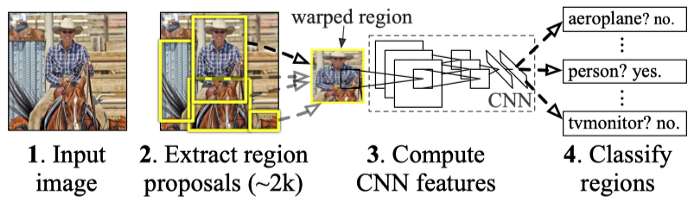
\includegraphics[scale=0.5]{./img/rcnn.png}
    \caption{R-CNN Aufbau, \cite[S.2]{Girshick.2016}}
    \label{fig:rcnn}
\end{figure}

Abbildung \ref{fig:rcnn} zeigt den Aufbau des zuerst beschriebenen \ac{R-CNN}. Hierbei greifen drei Module ineinander \cite[S.3-6]{Girshick.2016}. Die Aufgabe des ersten Moduls ist die Erzeugung von Region Proposals (dt. Region Vorschlag) für das Bild. Es sollen also die Regionen markiert, bzw. ausgegeben werden in dennen sich mögliche Objekte befinden. Hierfür wurde auf die Selective Search \cite{Uijlings.2013} zurückgegriffen. Die Autoren verweisen auf die Schwierigkeit mit Überlappungen, also dem sich nur teilweise in einer Region befindenden Objekt. Diese Probleme wurden durch das Einführen eines treshholds von 0.3 \cite[S.5]{Girshick.2016}. Alle Regionen, die unter diese Grenze fallen werden als negativ betrachtet und werden somit nicht weiter verarbeitet.
Auf den gefundenen Regionen aufbauend arbeitet nun ein \ac{CNN}, im speziellen eine Caffe Implementation desselben \cite{Jia.21.06.2014}. Die gewünschte Ausgabe dieses \ac{CNN}s ist ein Feature Vektor, der an das letzte Module, einer Anzahl \ac{SVM}, übergeben wird. Es handelt sich dabei um klassenspezifische \ac{SVM}, die im späteren Verlauf eine weitere Rolle übernehmen. Bei Erkennen eines Objekts wird durch den Output der \ac{SVM} eine klassenspezifische Bounding Box um das Objekt gelegt, um die genaue Lokalisierung zu verbessern \cite[S.12f.]{Girshick.2016}.
Wie bereits beschrieben wurde der ursprüngliche Ansatz der \ac{R-CNN} mehrfach verbessert, über das Fast \ac{R-CNN} \cite{Girshick.30.04.2015} hin zum Faster \ac{R-CNN} \cite{Ren.04.06.2015}. Diese zielen vornehmlich auf die schnellere Berechnung und Verarbeitung der Region Proposals, die den zeitaufwendigsten Schritt der \ac{OD} darstellt \cite[S.1]{Ren.04.06.2015}. Die Verarbeitungszeit wird bei Fast \ac{R-CNN} reduziert, indem nicht mehr für jede Region Proposal durchführen muss, es werden Berechnungen geteilt. Das \ac{CNN} nimmt als Input das Bild und alle Region Proposals und erzeugt darauf aufbauend eine Feature Map, die für die Erzeugung der Feature Vektoren benutzt wird. \cite[S.2f.]{Ren.04.06.2015}. Faster \ac{R-CNN} verbessert die Gesamtlaufzeit weiter, indem die Berechnungzeit der Region Proposals verringert wird. Hierfür werden Regional Proposal Networks genutzt, die als Ergänzung der bisher benutzten \ac{CNN} dienen können \cite[S.3f.]{Ren.04.06.2015}. Durch dieses Modul kann auf dem verwendeten Setup der Autoren eine \ac{OD} bei 5 \ac{FPS} durchegführt werden.

\subsection{Single Shot MultiBox Detector}

Trotz der erreichten Verbesserungen der \ac{R-CNN} erreichen diese dennoch keine zufriedenstellende Performance für Echtzeit \ac{OD}. Dies gelingt erst mit den YOLOv1 Netzwerken (siehe Kapitel \ref{sec:yolo-einführung}) und den \ac{SSD}. Letztere liefern eine etwa 74 prozentige Accuracy bei 59 \ac{FPS} \cite[S.2]{Liu.08.12.2015} und übertreffen damit Faster \ac{R-CNN} bei weitem, sowie YOLOv1. Diese Verbesserung wird erreicht, indem unter anderem auf die "bounding box proposals" \cite[S.2]{Liu.08.12.2015} verzichtet wird. Umgesetzt wird dies duch den Einsatz kleiner convolutional filter die Objektkategorien, und die dazu passenden bounding box locations, predicten. Die Filter werden auf verschiedenen Feature Maps im ganzen Verlauf des Netwerkes eingesetzt, so dass eine multipel skalierte Prediction erreicht wird \cite[S.2]{Liu.08.12.2015}.

\begin{figure}[H]
    \centering
    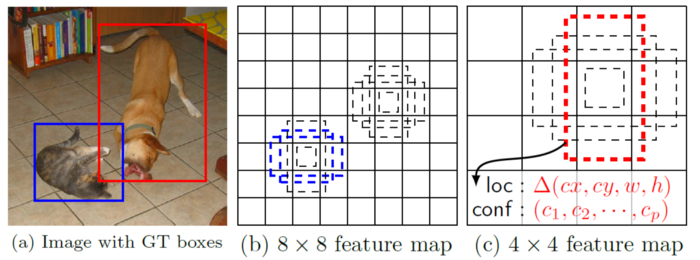
\includegraphics[scale=0.5]{./img/ssd.png}
    \caption{SSD framework, \cite[S.3]{Liu.08.12.2015}}
    \label{fig:ssd}
\end{figure}

Abbildung \ref{fig:ssd} zeigt ein Beispiel für die Bais Funktionsweise eines \ac{SSD}. Als Input wird ein Bild genommen auf dem Boxen für verschiedene Klassen (hier Hund und Katze) vermerkt sind. In Feature Maps mit verschiedenen Skalen (hier 8x8 und 4x4) sollen die Boxen des Bildes predicted werden. Dafür wird eine kleine Anzahl (hier 4) vordefinierter bounding boxen über das Bild gelegt und davon ausgehend predicted welche Klasse sich in ihr befindet, bzw. eine Anpassung der Dimensionen der Bounding Box vorgenommen \cite[S.3f.]{Liu.08.12.2015}.

\subsection{You Only Look Once}\label{sec:yolo-einführung}

Im Gegensatz zu herkömmlichen \ac{OD} Systemen verzichtet \ac{YOLO} auf langwierige Vorberechnungen, wie z.B. bei \ac{R-CNN} die Region Proposals. Das zuvor angesprochene \ac{SSD} arbeitet nach dem selben Prinzip, wurde jedoch erst nach der originalen YOLO Vorstellung beschrieben. Aus diesem Grund soll in diesem Kapitel zunächst auf die Basis Funktionsweise eines \ac{YOLO} Netzwerks eingegangen werden, bevor sich mit dem aktuellen (und für dieses Seminar verwendete) YOLOv3 beschäftigt wird.

\begin{figure}[H]
    \centering
    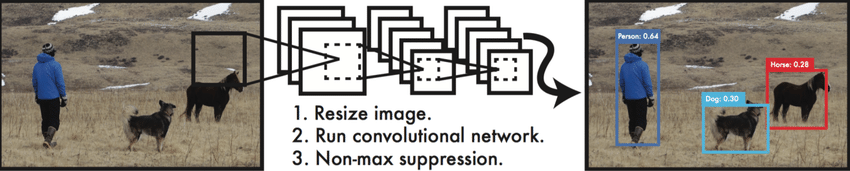
\includegraphics[scale=0.5]{./img/yolo.png}
    \caption{YOLO Detection System, \cite[S.1]{Redmon.08.06.2015}}
    \label{fig:yolo}
\end{figure}

Abbildung \ref{fig:yolo} zeigt dabei vereinfacht die Funktionsweise auf. Das Eingabebild wird auf eine vorgegebene Größe geändert, bevor in einem \ac{CNN} simultan verschiedene Bounding boxes, sowie die zugehörigen Klassenwahrscheinlichkeiten erzeugt werden \cite[S.1]{Redmon.08.06.2015}
\ac{YOLO} betrachtet dabei das Bild im Ganzen, womit auch kontextuelle Klasseninformationen in die \ac{OD} miteinbezogen werden können \cite[S.1f.]{Redmon.08.06.2015}. Dies unterscheidet es vom \ac{R-CNN}, das im Hintergrund mehr als doppelt so oft falsche Objekte erkennt als \ac{YOLO} \cite[S.2]{Redmon.08.06.2015}.
[Hier fehlt noch die genaue Funktionsweise des YOLO Netzwerks, sowie die Änderungen in YOLOv3 und warum sich für YOLO entschieden wurde]


\section{YOLO Implementierung}\label{sec:yolo}

\subsection{Vortrainierte Modelle}

Für die Implementierung der \ac{YOLO} \ac{OD} wurde auf vortrainierte config und weight Dateien zurückgegriffen. Redmon et all. stellen diese auf ihrer \href{https://pjreddie.com/darknet/yolo/}{Website} \cite{RedmonJosephFahradiAli.2020} zur Verfügung.
Für diese Arbeit wurde YOLOv3, sowie YOLOv3-tiny verwendet.
In der dieser Arbeit beigefügtem Git Repository befindet sich die \ac{OD} in der Datei /AutonomousCar/main/object-detectiion/object-detection.py. In der nun folgenden Erklärung werden kurze Code Abschnitte verwendet, für eine komplette Durchsicht des Codes sei auf die oben genannte Datei verwiesen.
Die Implementierung basiert dabei auf Tutorials von Adakane \cite{DarshanAdakane.2019, DarshanAdakane.2019b}.
Die vortrainierten weights / cfgs basieren auf den coco Datensatz (Z. 10). Wie bereits in Kapitel \ref{sec:yolo-einführung} dargelegt wird das Image auf eine bestimmte Größe, hier 416x416 skaliert (Z.3). Unser Code bietet die Möglichkeit (Zeile 7) zwischen den verschiedenen YOLO verisonen zu wechseln, was aufgrund der Performance auf dem Rapsberry Pi nötig ist. Auf diesen Punkt wird in Kapitel \ref{sec:performance} eingegangen. In Zeile 13 und 14 wird das vorverarbeitete Bild dem Netwerk übergeben. Als Rückgabe wird eine Liste der erkannten Objekte erwartet.

\begin{lstlisting}[language=Python]
...
# preprocess image
blob = cv2.dnn.blobFromImage(img_original, 1 / 255.0, (416, 416), 
swapRB=True, crop=False)

# load network
output_layers, net = load_yolo(tiny=tiny)

# load coco list
class_list = load_coco_names()

# detect objects
net.setInput(blob)
outs = net.forward(output_layers)
...
\end{lstlisting}

Diese Ergebnisse werden dann in zwei Funktionen (information-cal und information-draw) weiter verarbeitet. Information-cal (Datei ab Zeile 68), überprüft dabei für jedes Objekt in outs, ob es mit einer zufriedenstellenden Confidence (hier 0.5) erkannt wurde. Außerdem werden die Höhe, Breite, x- und y-Position der Bounding Box berechnet und gespeichert. Diese Box wird außerdem mit dem Objekt-Namen angereichert.
Daraufhin werden die Ergebnise der information-draw Funktion übergeben, die dann mithilfe von opencv in das Eingabebild eingezeichnet werden. opencv bietet dabei die Möglichkeit das Schriftbild zu verändern.

\begin{lstlisting}[language=Python]
...
for i in range(len(boxes)):

    if i in indexes:
    
        x, y, w, h = boxes[i]
        label = str(class_list[class_ids[i]])
        full_label = label + ", " + str(round(confidences[i] * 100, 2))
        color = colors[class_ids[i]]
        cv2.rectangle(img, (x, y), (x + w, y + h), color, rec_width)
        cv2.putText(img, full_label, (x, y -5), font, txt_height,
        color, text_width)
...
\end{lstlisting}

Das oben gezeigte beschreibt die Erkennung für jeweils ein Bild. Dies kann auf einen Videostream (z.B. Webcam, hier Pi-Camera) umgeschrieben werden, indem jeder einzelne der von der Kamera aufgezeichneten Frames diesen Prozess durchläuft.

\subsection{Individuell trainiertes Modell}

Aufgrund des Modellmaßstabes des Projekts wird das Auto auf keine Menschen treffen, die die \ac{OD} auslösen können.
Aus diesem Grund wurde versucht ein individuelles \ac{YOLO} Netzwerk zu trainieren, dass Playmobilmenschen erkennt. Im Folgenden sollen die dafür verwendeten Schritte beschrieben werden.
\begin{enumerate}
    \item Datenbeschaffung:
    Als Datenquelle wurde zunächst die PlaymoDB \cite{PlaymoDB.2020} nach passenden Bildern durchsucht. Abbild \ref{fig:playmo} zeigt ein Beispielbild. Hieran wird auch ein mögliches Hemmniss deutlich. Der überwiegende Teil der Bilder ist aus diesem Winkel und dieser Position aufgenommen worden, sodass fraglich bleibt wie gut das Training funktioniert.
    
    \begin{figure}[H]
        \centering
        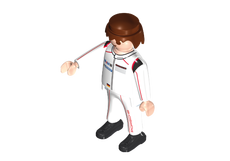
\includegraphics[scale=0.5]{./img/playmo.jpg}
        \caption{PlaymoDB Bild}
        \label{fig:playmo}
        \\ Quelle: https://playmodb.org/cgi-bin/showpart.pl?partnum=302000200404
    \end{figure}
    
    Alternativ dazu wurden eigene Bilder (im Github Repositorry unter ...) verwendet.
    \item Labeling:
    Ein zentraler (und zeitaufwendiger) Punkt des Trainings ist das Labeling der zuvro beschafften Bilder. Dieses geschieht in unserem Fall über das pip labeling Tool labelImg (siehe Abbildung \ref{fig:label}. Hierbei werden die Objekte (Playmobilfiguren) mit einer passenden Bounding Box versehen. Diese Informationen werden in einer txt Datei gespeichert im Format <ClassID> <x-Zentrum> <y-Zentrum> <Breite> <Höhe>.
    
    \begin{figure}[H]
    \centering
    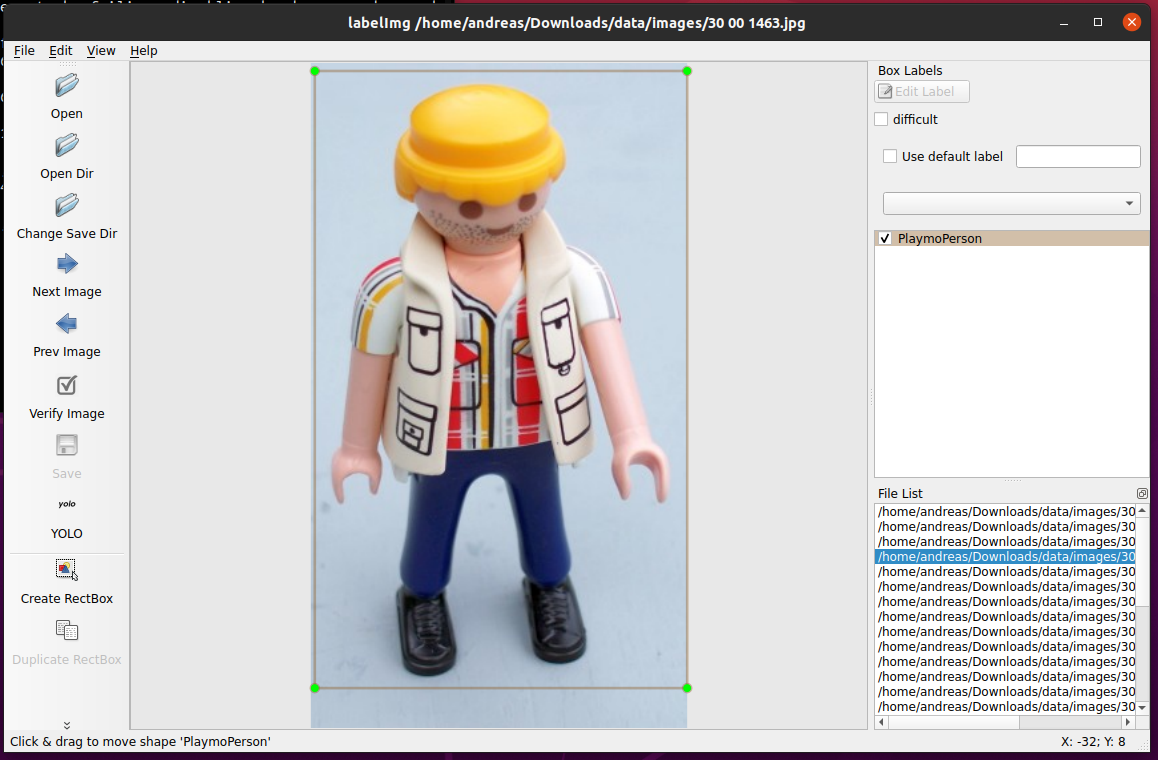
\includegraphics[scale=0.2]{./img/label.PNG}
    \caption{LabelImg Anwendung}
    \label{fig:label}
    \end{figure}
    
    \end{enumerate}
    \item Training:
    Für das Training wird auf ein Tutorial, sowie ein bereitgestelltes Google Colab Notebook zurückgegriffen \cite{Rafi.2019}. Erwähnt seien die nötigen Anpassungen in den cfg Dateien (ob \ac{YOLO} oder tiny \ac{YOLO}). Hierfür müssen in den YOLO Layern, sowie dem jeweils vorgelagerten Conv Layer Veränderungen vorgenommen werden.
    \begin{lstlisting}
    ...
    [convolutional]
    size=1
    stride=1
    pad=1
    filters=18
    activation=linear
    
    [yolo]
    mask = 3,4,5
    anchors= 5.80289956, 11.72601733, 7.61052314, 11.16109429, 11.2596055, 12.61, 11.698908, 12.6685, 12.263004, 12.584, 12.816258, 12.038
    classes = 1
    num = 6
    jitter=.3
    ignore_thresh = .7
    truth_thresh = 1
    random=1
    ...
    \end{lstlisting}
    Diese betreffen die filters in Zeile 6, diese müssen entsprechend der Formel,
    \begin{equation}
        filters = (Klassenanzahl+5) * num / 2
    \end{equation}
    also: filters = (1+5)* 6/2 = 6*3 = 18, gesetzt werden.
    Außerdem muss in Zeile 12 die Anzahl der Klassen angepasst werden.
    Nach diesen Anpassungen kann das Colab Notebook ausgeführt werden, welches nach einer definierten Anzahl an Trainingsschritten die Gewichte ausgibt.

\subsection{Performance}\label{sec:performance}

[Über Performance von normalen und tiny yolo schreiben]

\section{Distanz Errechnung}\label{sec:distance}

Mithilfe von OpenCV ist es möglich den Abstand zu einem erkannten Objekt in einem Bild relativ zur Kamera zu messen.
Hierfür wird auf ein Tutorial von Rosebrock zurückgegriffen \cite{AdrianRosebrock.2015}.
Die Berechnungen basieren auf der Dreiecks Ähnlichkeit (triangle similarity). Diese besagt in unserem Fall im Groben, dass wir ausgehend von einem Objekt in einem Foto, dessen Weite und Abstand bekannt sind, die Brennweite (focal length) berechnet werden kann. VOn dieser ausgehend kann dann für ein neues Objekt, dessen Pixelweite bekannt ist, der Abstand zur Kamera berechnet werden. Das neue Objekt, bzw. die neue Breite sind im Fall dieses Projektes die Weite der Bounding Box eines bestimmten Objekts.
Für dieses Modell wurde als Kalibrierungsmaßstab eine Soundbox mit 16cm Breite und einem 50cm Abstand zur Kamera gewählt. Mithilfe des in Kapitel \ref{sec:greyscaling} beschriebenen Grayscalings, sowie einer opencv Funktion, die es erlaubt Konturen zu finden und zu extrahieren (cv2.findContours()) kann die Pixelweite der Soundbox extrahiert werden.

\begin{figure}[H]
    \centering
    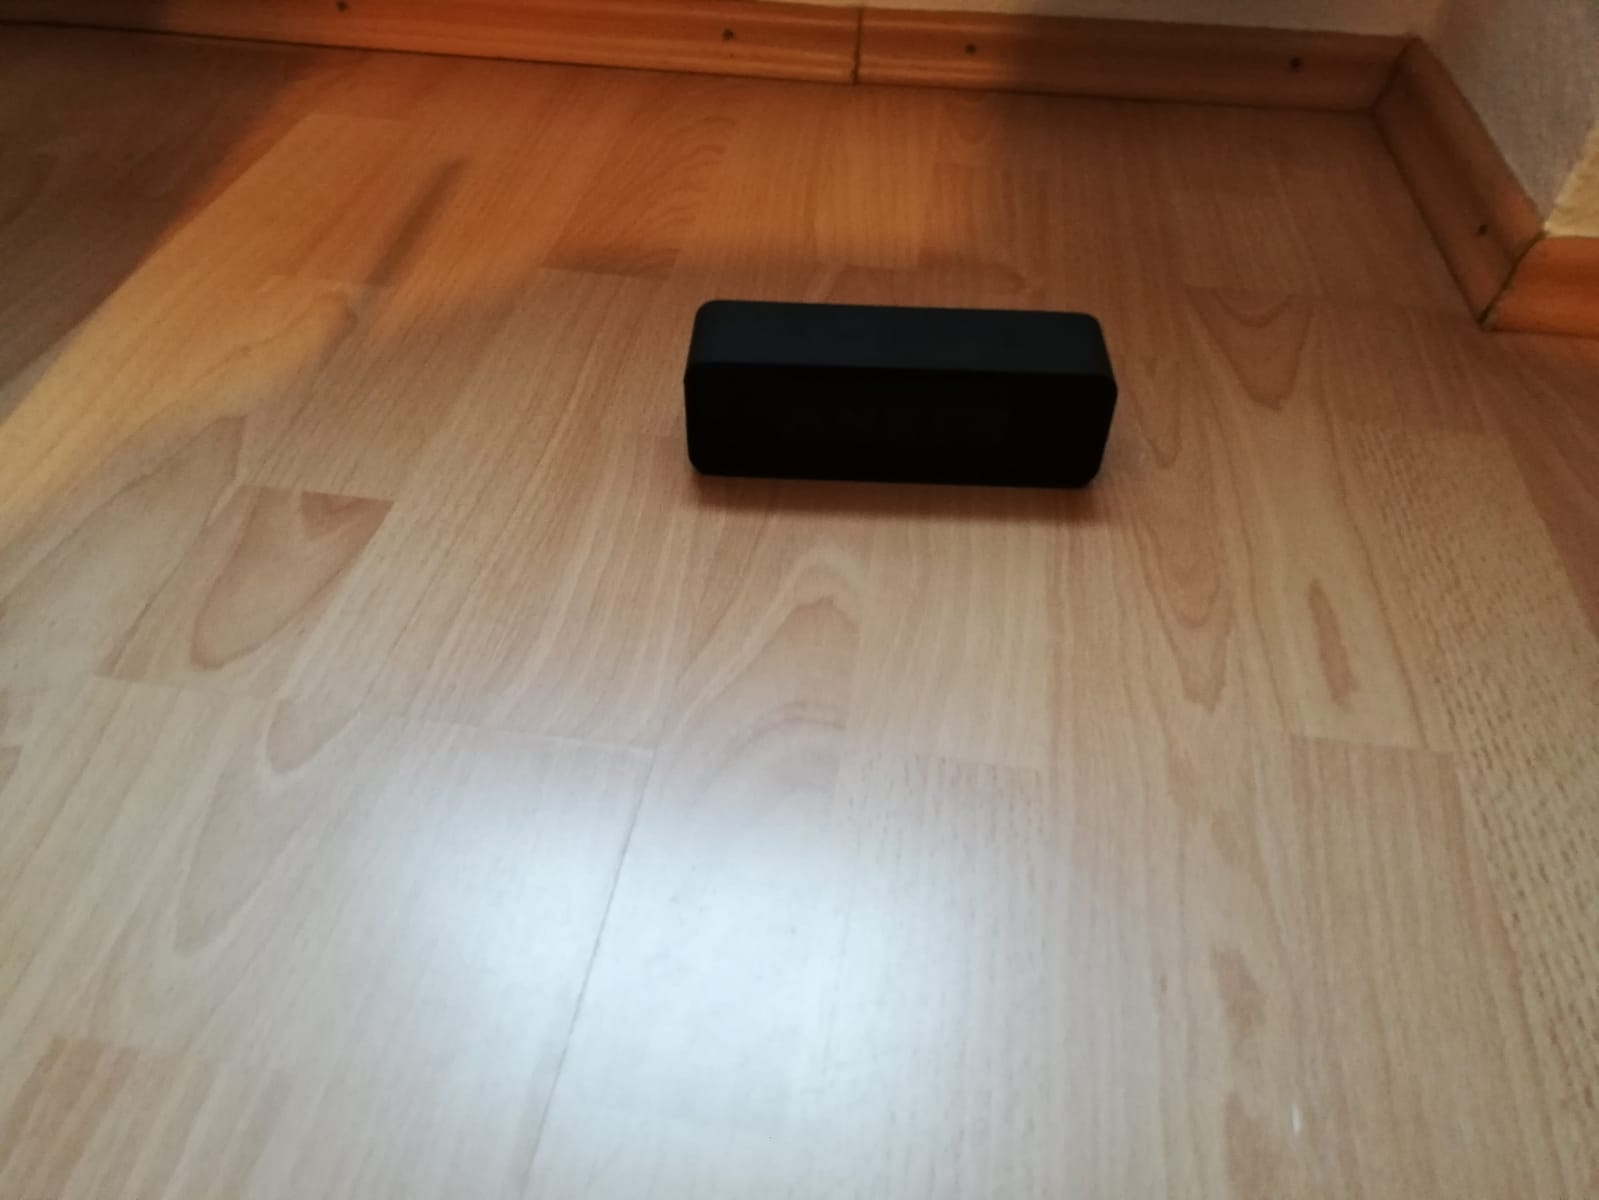
\includegraphics[scale=0.1]{./img/marker.jpg}
    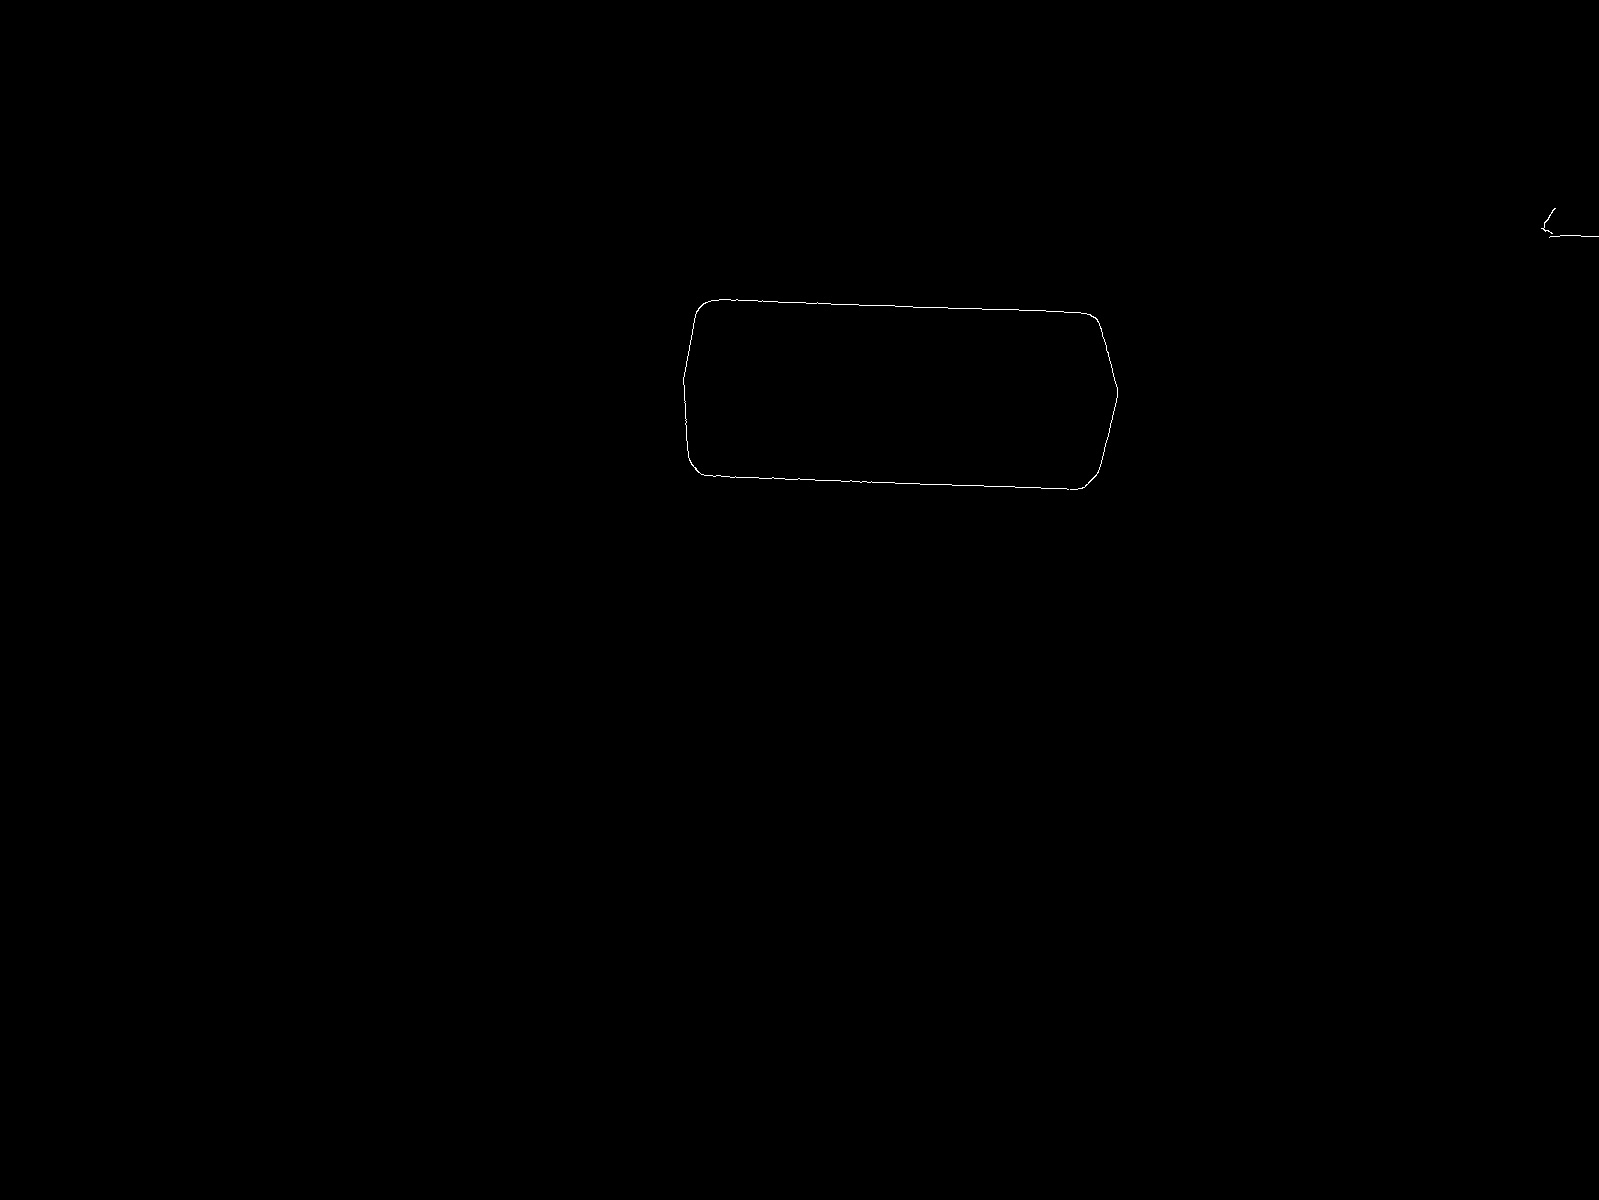
\includegraphics[scale=0.1]{./img/marker_gray.jpg}
    \caption{Marker (Original links, Kontur rechts)}
    \label{fig:marker}
\end{figure}

Die focal length errechnet sich durch:
\begin{equation}
    focalLength = (marker-pixel-width * marker-distance) / marker-width
    \label{equ:focalLength}
\end{equation}

Hiervin ausgehend kann die Distanze zu Objekten errechnet werden:
\begin{equation}
    distance = (marker-width * focalLength) / object-width
    \label{equ:distance}
\end{equation}

Zu beachten ist, dass die focal Length kamera, sowie Winkelspezifisch ist. Es ist somit auf ein aktuelles Kalibrierungsfoto zu achten.

In unserem Projekt soll mithilfe der Distanz Messung ein Call to Action erreicht werden. In der zugehörigen Funktion check-reation (Z. 106) wird in einer List festgelegt bei welchen Klassen die Distanz gemessen werden soll, z.B. person. Sobald eine Person erkannt wird, wird für diese auch laufend die Distanz errechnet. Im folgenden kann dann an das Auto ausgegeben werden zu stoppen, falls sich eine Person unterhalb eines bestimmten Abstands zur Kamera (und damit zum Auto) befindet.
\chapter{Raspberry Pi Car}
%https://www.matec-conferences.org/articles/matecconf/pdf/2017/39/matecconf_cscc2017_02025.pdf

%https://www.wseas.org/multimedia/journals/power/2017/a465916-072.pdf


\section{Hardware}
Für die Umsetzung des Projekts wird ein 1:10 ferngesteuertes Modellauto und ein Raspberry PI 3B+ mit Kameramodul verwendet. Auf die genaue Verwendung der genannten Komponnenten wird im Weiteren eingegangen. 

\subsection{Raspberry Pi}
\begin{figure}
\centering
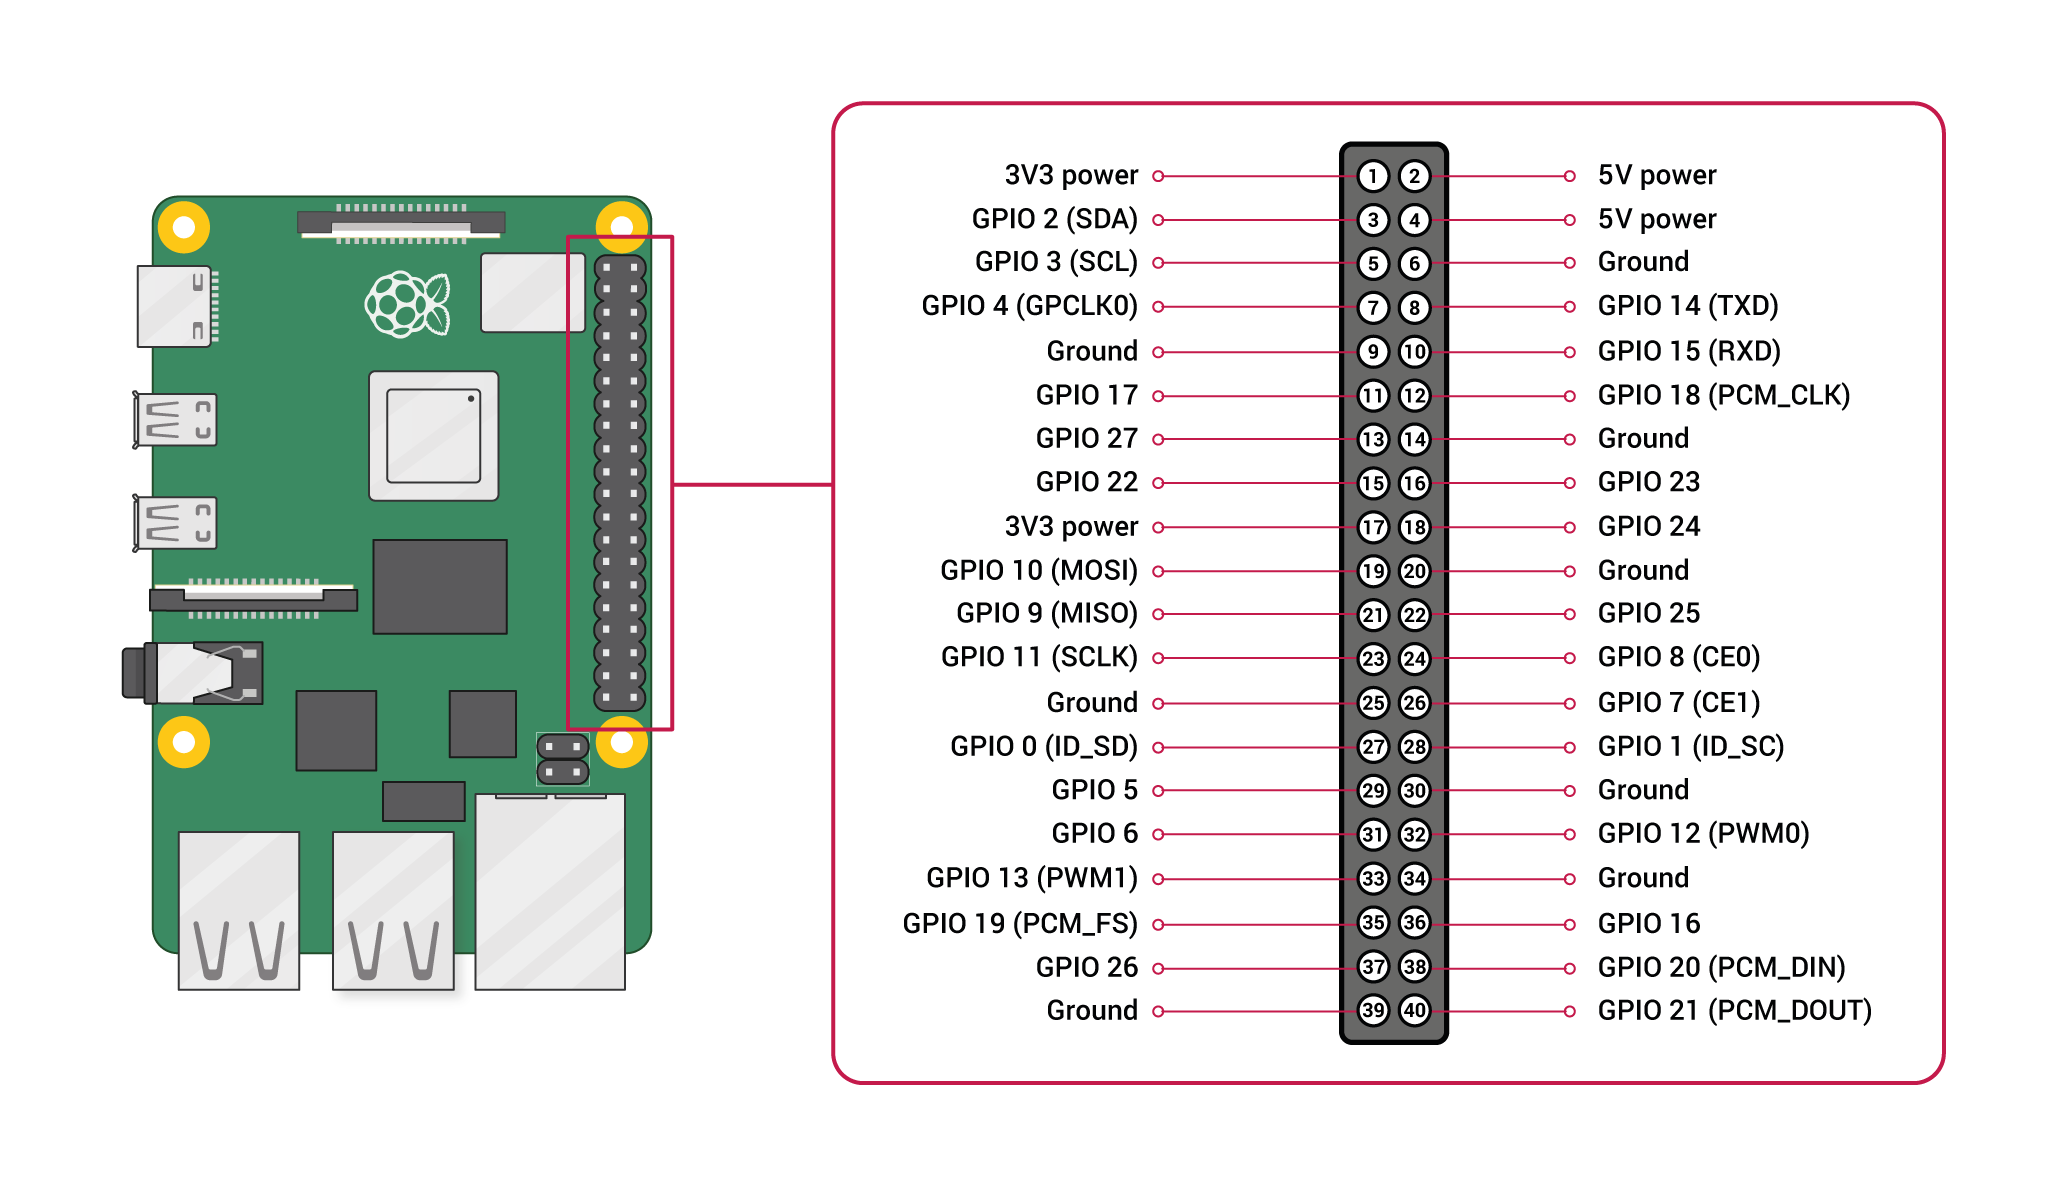
\includegraphics[width=\textwidth]{\imagedir/Raspberry.png}
\caption{Raspberryboard \autocite[VglRaspberrboard]{https://www.raspberrypi.org/documentation/usage/gpio}} 
\end{figure}
Ein \ac{Pi} ist ein Minicomputer mit Betriebssystem in Kreditkartengröße. Er verfügt unter anderem über USB-Anschlüsse, einen HDMI-Port, sowie einen Anschluss für ein Kameramodul. Desweiteren verfügt der \ac{Pi} über \ac{GPIO}-Ports die über Programmiersprachen, wie zum Beispiel Python mit den entsprechenden Bibliotheken, angesteuert werden können. 

Für dieses Projekt wird Raspberry Pi OS als Betriebssystem auf einer 8 Gb microSD und eine 10.000 mAh Powerbank zum Betreiben des \ac{Pi}'s genutzt.

Der \ac{Pi} bildet das Herzstück des \ac{SELMA}. Mit Hilfe des Kameramodul werden Bilder aufgenommen, die durch die Softwarekomponenten Lanedetection und Objectdetection ausgewertet werden, um mit deren Ausgaben das Modellauto zu steuern.

Die Programmierung findet hauptsächlich außerhalb des \ac{Pi}'s auf den Laptop's der Gruppenteilnehmer statt. Um den Code auf den \ac{Pi} zu spielen, wird dort das Github des Projekts gecloned und fortlaufend aktualisiert. Zur Erleichterung bei kleinen Änderungen auf dem \ac{Pi} kommen eine USB Maus, Tastatur und ein externer Monitor zum Einsatz.

\subsection{Modellauto}
Das Modellauto besteht aus den Komponenten: Lenkservo, Funkfernsteuerung, Empfänger, Motor, Fahrtenregler und Akku. Die Steuerung funktioniert im eigentlichen Sinne über die Funkfernsteuerung welche Signale an den Empfänger sendet. Dieser wird über die Verbindung des Fahrtenreglers mit Strom versorgt und versorgt seinerseits den Lenkservo mit Strom. Die Verbindung zu Lenkservo und Fahrtenregler besteht aus jeweils drei Adern. Zwei dienen der Stromversogung, wie bereits beschrieben, die dritte Ader dient der Ansteuerung der beiden Komponenten. Über diese Ader werden \ac{PWM} Signale in einer bestimmten Frequenz übermittelt. \ac{PWM} ist eine digitale Modulationsart, bei der in gegebener Frequenz ein Intervall in bestimmter Dauer übermittelt.

\begin{figure}[H]
\centering
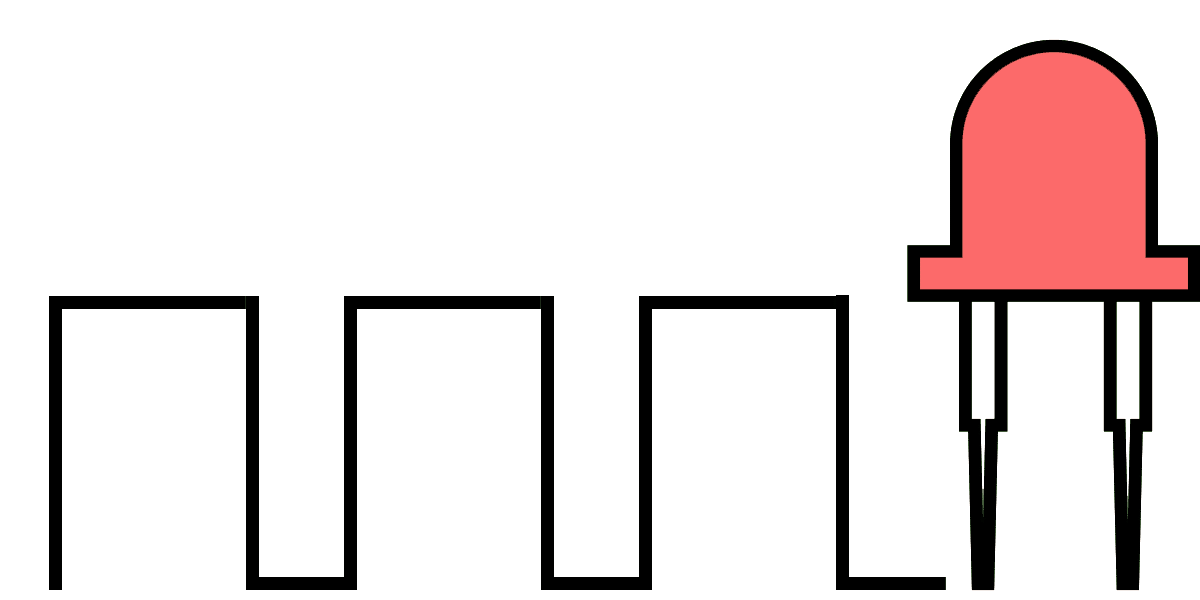
\includegraphics[width=\textwidth]{\imagedir/PWM.png}
\caption{Raspberryboard \autocite[VglRaspberrboard]{https://www.raspberrypi.org/documentation/usage/gpio}} 
\end{figure}

Je nach Intervalldauer gibt beispielsweise der Fahrtenregler Gas beziehungsweise lenkt das Lenkservo.

\subsection{Verkablung}
Um das Modellauto mit dem \ac{Pi} zu steuern, muss die Übermittlung der \ac{PWM} Signale vom \ac{Pi} geschehen. Um dies zu realisieren, wird der \ac{Pi} zwischen den Empfänger und den Lenkservo beziehungsweise dem Fahrtenregler eingelötet. Um die \ac{PWM} Signale vom \ac{Pi} zu übermitteln, muss jeweils für Lenkservo und Fahrtenregler, ein Minuskabel und die dritte Arder, für die Signalübertragung, mit dem \ac{Pi} anstatt dem Empfänger verbunden. Im folgenden ist die Verbindung zwischen allen Komponenten visuell dargestellt:
\begin{figure}[H]
\centering
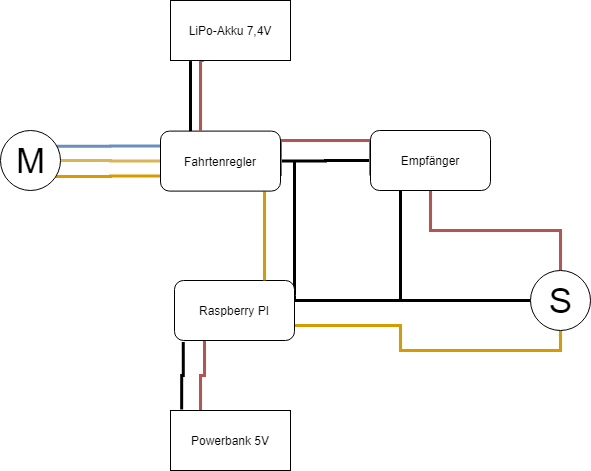
\includegraphics[width=\textwidth]{\imagedir/Schaltplan.jpg}
\caption{Raspberryboard\autocite[Vgl https://www.raspberrypi.org/documentation/usage/gpio]{}} 
\end{figure}

\subsection{Ansteuerung der \ac{GPIO}-Pins mit Python}\label{ss:Ansteuerung}
Für die Umsetzung der Ansteuerung wird die RPi.GPIO Bibliothek und die Pins 33 und 35 für Fahrtenregler und Lenkservo genutzt. Die \ac{PWM} Signale werden in einer 50 Hertz Frequenz übermittelt. Hierbei muss besonderes Augenmerk auf die korrekte Frequenz gelegt werden, da sonst die Elektronik des Lenkservos beziehungsweise des Fahrtenreglers durchbrennen kann. Dies ist bei der Umsetzung des Projektes leider zweimal mit Lenkservos geschehen. Im Folgenden werden die Kernbestandteile der \ac{PWM}-Ansteuerung erklärt. Die volle Ansteuerung ist im Anhang unter \ref{c:steeringcontroll} zu finden.

\begin{lstlisting}[language=Python]
IO.setmode(IO.BOARD)
IO.setup(35,IO.OUT)
steering =IO.PWM(35,50)
steering.start(0)
\end{lstlisting}
Mit den obigen Befehlen wird die Ansteuerung des \ac{PWM}-Pin 35 mit einer 50 Hertz-Frequenz initiiert. Die Aktivintervalldauer (duty cycle) wird dabei auf 0 gesetzt.

\begin{lstlisting}[language=Python]
steering.ChangeDutyCycle(10)
steering.stop()
\end{lstlisting}
Mit der Funktion ChangeDutyCycle kann die Dauer des Aktivenintervalls (duty cycle) verändert werden. In diesem Beispiel wird die Zeit des Aktivenintervalls auf 10\% der Intervalldauer gesetzt. Mit der Funktion stop wird die Ansteuerung des entsprechenden \ac{GPIO}-Pins gestoppt.


\section{Steuerung des Modellautos}

%https://link.springer.com/chapter/10.1007/978-1-4842-5174-4_1
Introduction to machine learning (ML) with the Raspberry Pi (RasPi)

Für die Steuerung des Modellautos wird das run\_car.py Skript genutzt. Dieses nutzt die Kamera um ständig Bilder aufzunehmen und diese zur Steuerung auszuwerten. Dazu werden die bereits erklärten Funktionen aus object- und lane\_detection genutzt. Darüber hinaus wird ein Car-Objekt erzeugt, mit dem das Modellauto angesteuert werden kann. Dies wurde in \ref{ss:Ansteuerung} erläutert.
\newline
Die Auswertung der Kamerabilder werden in einer While-Schleife durchgeführt. Dazu wird zu Beginn der While-Schleife ein Bild mit der Kamera erstellt. Dieses wird dann, falls kein Thread zur Objekterkennung läuft, an einen neune Thread zur Objekterkennung übergeben. Dieser läuft asynchron und blockiert nicht den weiteren Ablauf und die Auswertung zur Steuerung des Autos. Nach dem, falls notwendig, der Objekterkennungsthread gestartet wurde, wird das Bild mit Hilfe der lane_detection Funktion aus dem lanedetect_steer Skript ausgewertet. Die Funktion gibt einen Anweisung zur Steuerung des Modellautos zurück. Diese Anweisung wird genutzt um mit der Steer-Methode das Modellauto zu steuern. Der Objekterkennungsthread liefert einen Boolean zurück. Sollte die Booleanrückgabe True sein, wird das Auto angehalten und erst wieder gestartet, wenn die Rückgabe False ist. 

% Fazit und Ausblick
% !TEX root =  master.tex
\chapter{Zusammenfassung}

\nocite{*}

Dieses Kapitel enthält die Zusammenfassung der Arbeit mit Fazit und Ausblick.

\section{Fazit}

...

\section{Ausblick}

...


%%%%%%%%%%%%%%%%%%%%%%%%%%%%%%%%%%%

\initializeAppendix

%%%%%%%%%%%%%%%%%%%%%%%%%%%%%%%%%%%
% ANHÄNGE
%
% @stud: einzelne Anhänge bearbeiten und eigene Anhänge hier einfügen 
%
% !TEX root =  master.tex
\chapter{Steeringcontroll}\label{c:steeringcontroll}
UPDATEN!
\begin{lstlisting}[language=Python]
import RPi.GPIO as IO
import time

class Car():
    def __init__(self):
        #setup the raspberry for PWM on Pin 35
        IO.setwarnings(False)
        IO.setmode(IO.BOARD)
        IO.setup(35,IO.OUT)
        #starting pin controll
        self.steering =IO.PWM(35,50)
        self.steering.start(0)
        #set steerendpoints
        self.FULL_LEFT=10
        self.STRAIGHT=8
        self.FULL_RIGHT=6
        #get steeringrange from straightpoint
        self.LEFT=self.FULL_LEFT-self.STRAIGHT
        self.RIGHT=self.STRAIGHT-self.FULL_RIGHT

    def __del__(self):
        self.steering.stop()

    def steer(self,steeringrate):
            if steeringrate == 0:
                self.steering.ChangeDutyCycle(self.STRAIGHT)    
            elif steeringrate > 0:
                steeringrate=self.STRAIGHT + self.LEFT * steeringrate            
                if steeringrate > self.FULL_LEFT:
                    steeringrate=self.FULL_LEFT
                self.steering.ChangeDutyCycle(steeringrate)
            elif steeringrate < 0:
                steeringrate=self.STRAIGHT - self.RIGHT * abs(steeringrate)
                if steeringrate < self.FULL_RIGHT:
                    steeringrate=self.FULL_RIGHT
                self.steering.ChangeDutyCycle(steeringrate)
\end{lstlisting}

\chapter{Run\_car}\label{c:run_car}
\begin{lstlisting}[language=Python]
camera = VideoCamera(flip=False)
car = controll_car.Car()

object_detection_thread = threading.Thread(target=object_detection.detect_webcam_delay, args=(1,))
input("Hit Enter to run the car")
car.run()
object_output=None
outputcounter=0
while True:
    frame = camera.get_frame()
    try:
        if not object_detection_thread.is_alive():
            print("objectdetection started")
            object_detection_thread = threading.Thread(target=object_detection.detect_webcam_delay, args=(1,))
            object_output= object_detection_thread.start()
        if object_output == True:
            car.stop()
        elif object_output == False:
            car.run()
        frame2, canny, steering=lanedetect_steer.lane_detection(frame,"indoor")
        car.steer(steering)
    except Exception as e:
    	print(e)
        print("steeringerror")
\end{lstlisting}
%%%%%%%%%%%%%%%%%%%%%%%%%%%%%%%%%%%

\singlespacing

%%%%%%%%%%%%%%%%%%%%%%%%%%%%%%%%%%%
% LITERATURVERZEICHNIS
% 
% @stud: Literaturverzeichnis in Datei bibliography.bib anpassen 
%
\initializeBibliography
%%%%%%%%%%%%%%%%%%%%%%%%%%%%%%%%%%%

\addcontentsline{toc}{chapter}{Index}
\printindex

\end{document}
